Figure \ref{fig:scnn-fc} shows the conceptual and theoretical framework to be used in the study. A dataset is first obtained for the study, specifically a food dataset coming from the Food-101 database \cite{bossard-2014}. The dataset is composed of 101000 food images classified into 101 classifications. The huge amount of samples justifies the use of a deep learning model. After gathering the data needed for the study, it will be split into the train and test sets, specifically, using the 75-25 percent split for the training and testing phase, respectively. All of the instances from both sets will be subjected to resizing, specifically to a 224 x 224 size since this is the required size of the model. After that, each instance will be converted into two color spaces specified in the experiment. This is such that for each sample, two color spaces are generated, for instance, image A is converted into HSV and LAB color spaces. After the conversion, each converted instance is rescaled to [0, 255] value range and then normalized to [0,1]. The normalized instance is again converted to the [0, 255] value range since this is the required input for our model. Additional data augmentation techniques are also applied for the model to be more robust and effective. The data augmentation is only triggered in the training phase of the model. The train set output of preprocessing the inputs can now be fed into the proposed model. The proposed structure is a Siamese CNN network with a pre-trained EfficientNet model, such as EfficientNetB0. The proposed model is fine-tuned to adapt to the food image classification problem. In the training phase, two different color space inputs are required for the Siamese network. An Adam optimizer will be used as well as a categorical focal loss loss function. After the training, the trained model will now be subjected to testing using the test set taken from the dataset. The same with the training phase, the testing phase will also require two color space inputs and will undergo the same preprocessing except for the data augmentation technique. The testing phase will measure the Top-1\% and Top-5\% accuracy. This will help in performing a comparison of the proposed model as well as models from the related studies. Finally, if the best model is achieved, it will be implemented on a web-based application to be deployed for real-world applications.
\begin{figure}[h]
 	\centering
	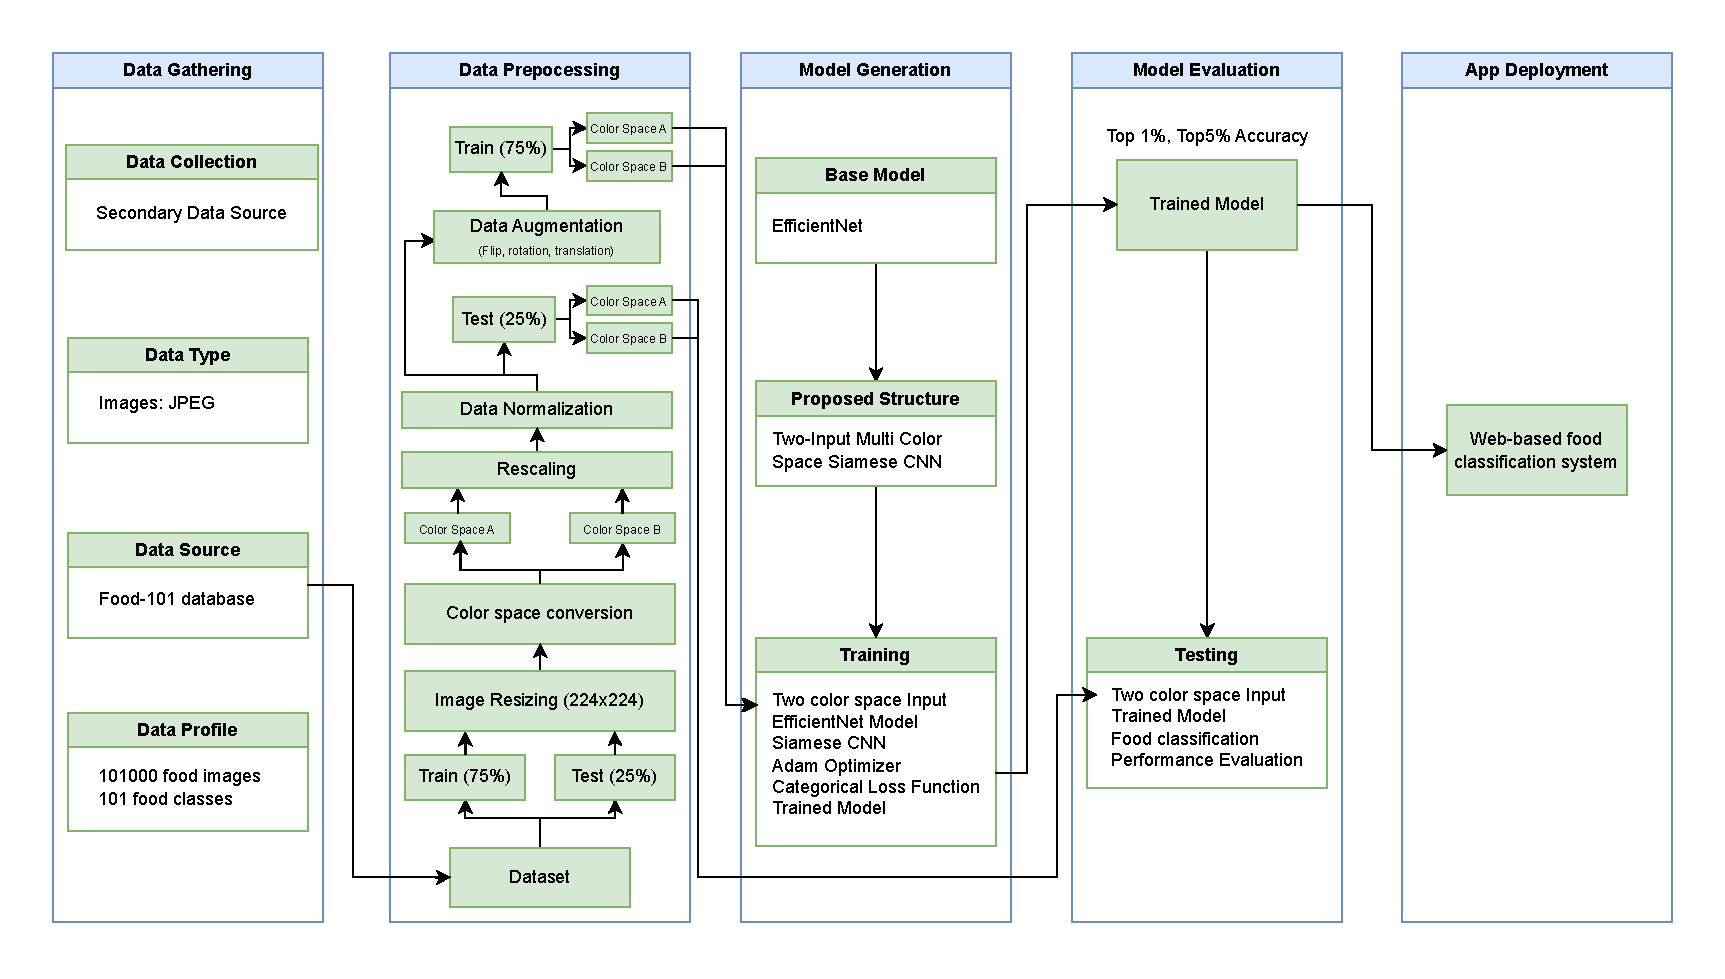
\includegraphics[width=1.15\textwidth]{graphics/images/scnn-fc-concept.pdf}
	\caption{Theoretical and Conceptual Framework}
	\label{fig:scnn-fc}
\end{figure}